\documentclass{article}
\usepackage{graphicx}
\usepackage{hyperref}
\title{Assignment 1}
\author{Tore Kjelds (tokj@itu.dk)}
\date{\today}

\begin{document}
\maketitle
Link to \href{https://github.com/tkjelds/BDSA_assignment01}{Github} 
\section*{C\#}
\begin{figure}[!htb]
    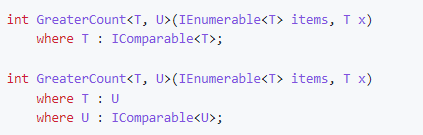
\includegraphics[scale = 0.7]{img/GreaterCount.png}
\end{figure}
In the first example, T has to implement the ICompareable interface. \\
In the second exapmle, T has to implement U, which implements ICompareable. \\ 
The first method, there is no certainty that the method can compare T and U, since only T has the interface implmented. \\
The second method, there is a certainty that the method can compare T and U, since they both implement the ICompareable interface. \\ 
\section*{Software Engineering}
\subsection*{Exercise 1}
\subsection*{Exercise 2}
\textbf{CoronaPas} would be a Interactive transaction-based application. I base this on the communication aspect between the server which verifies that the user has had vaccine. An argument could be made that this also falls in the category of systems of systems, since coronapas interacts with alot of different software systems. 
\\
\textbf{Git} would also be an Interactive transaction-based application. I base this on the transactions that occur when pulling and pushing. 
\subsection*{Exercise 3} 
\textbf{CoronaPas} would be considered a \textit{Generic product}, since it is offered on the open market to any one who wishes to download. An argument could be made that there are elements of \textit{bespoke} software, since it was commisioned by another company.
\\
\textbf{Git} Would be considered a \textit{Generic product}, since it is offered to any one, who wishes to use.
\subsection*{Exercise 4}
\textbf{Git} \\
I would argue that git focusses equally on the quality attributes. Git needs to be dependable, as if the service would be down, the companies using it would be losing money since the people working would'nt be able to push their commits to the pipeline. 
Efficiency is also an important attribute for git, since the amount of individual transaction occuring are very large, it is important to handle them efficiently.
Lastly, maintainability is also important for git, since the software needs to evolve with its users needs.
\textbf{CoronaPas} \\
I would argue that the Corona pas application leans more heavily towards security, since the application handles sensitive information about the user, and that specific legislations has strict requirements when it comes to handleing sensitive user data.
Of course Efficiency is also important, since most of the people in Denmark will be using the application, there will be a lot of transactions being made.
\textbf{Insulin pump control} \\
The insulin pump, would focus more heavily on the quality attribute dependability, since the result of having an inadequate dose or too frequent or infrequent dosages could lead to dangerous medical outcomes.
\subsection*{Exercise 5}
\begin{enumerate}
    \item Gitlet was written to show how Git works, not as a fully fledged software product. Meaning that it does not require the additional work of having a meaningfull architecture since it is a learning tool.
    \item You could look through the source code and look for file dependancies and look at just the overall file structure. Through the dependacies you could get an overview of the hierarchy.
    \item 
\end{enumerate}
\subsection*{Exercise 6}
\end{document}
s